\section{Randomness and Shuffling}
In the game of poker, the house does not wager against players, unlike other 
popular casino games, such as blackjack or roulette, but instead the usual 
method for online poker companies and indeed poker tables in real life to make 
money is the rake. 

The implementation of the rake varies between casinos and online poker
software. Some common ones are in the below table.

\begin{center}
    \begin{tabular}{l l}
    \toprule
    Mechanism           & Description                                               \\
    \midrule
    Pot Rake            & Percentage taken from the pot, per hand or betting round  \\ \addlinespace
    Dead Drop           & Fee paid by the player with the dealer button each hand   \\ \addlinespace
    Timed Rake          & Set fee collected every set interval of time              \\ \addlinespace
    Fixed Fee           & Fixed fee per hand                                        \\ \addlinespace
    Tournament Fee      & Entry fee to participate in poker tournaments             \\ \addlinespace
    Subscription Fees   & Players are charged a subscription fee to play            \\
    \bottomrule
    \end{tabular}
\end{center}

Finally, some games are rake free, instead generating revenue by driving
traffic to more profitable businesses. The software developed that this paper
is discussing is also rake free, due to being only for academic purposes.

However, despite companies being able to generate revenue in these ways, the
implementation of random number generation in poker software is a topic of
some interest. Possible issues include rogue employees writing malicious
code to give them or people connected to them beneficial cards, faulty code
allowing the random number generation to be exploited, and other schemes, such
as giving newer players or failing players better cards, to encourage them to 
continue using the companies platform, and generating revenue through rakes.

For these reasons, random number generation has been analysed and multiple
different shuffling algorithms or card picking algorithms have been
developed and contrasted for possible weaknesses. Two obvious approaches to 
selecting cards are:

\begin{itemize}
    \item Storing an array of all the cards and indexing this array in some way to take a card
    \item Shuffling an array in some way and taking the top item
\end{itemize}

\newpage

Multiple versions of both these algorithms have been implemented, using
different sources of randomness. Also developed is a GUI which can be launched
when the `--chooseshuffle' argument is given to the server, which allows
the card picking algorithm and random source to be altered mid game. 

\begin{figure}[H]
    \centering
    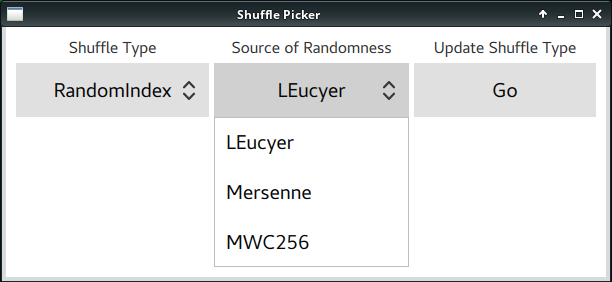
\includegraphics[width=0.8\linewidth]{../images/shufflepicker.png}
    \caption{The Shuffle Picker Window}%
    \label{fig:shufflepicker}
\end{figure}

Another program provides a similar interface but instead allows multiple hands 
to be drawn and the number of times each card was drawn displayed in a graph. 
This  allows us to easily see the effect of the different algorithms on the 
uniformness of the card distribution.

\begin{figure}[H]
    \centering
    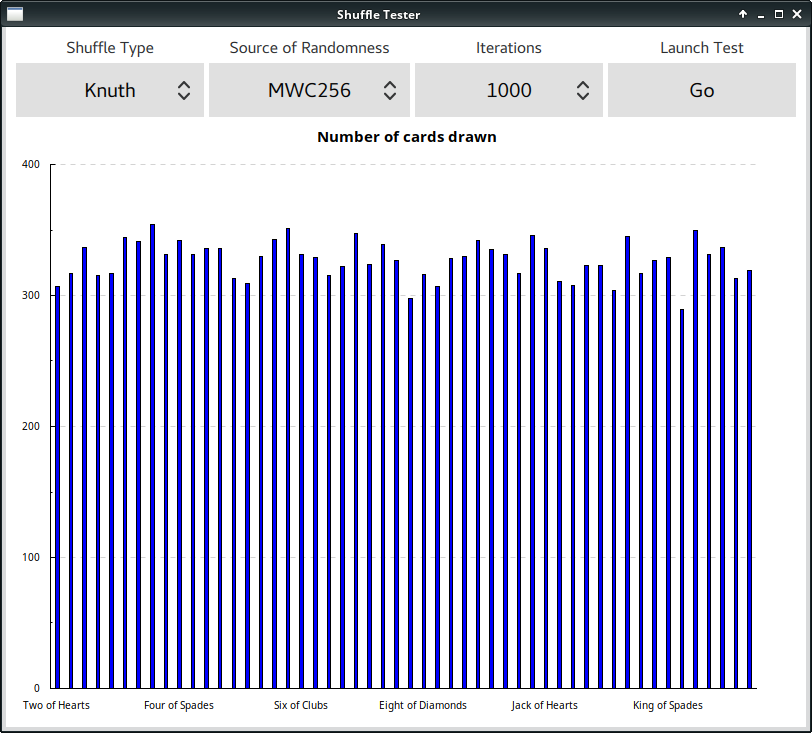
\includegraphics[width=0.8\linewidth]{../images/shuffletester.png}
    \caption{The Shuffle Tester Program}%
    \label{fig:shuffletester}
\end{figure}

The three sources of randomness used are:

\begin{itemize}
    \item Portable Combined Generator of L'Eucyer \parencite{leucyer1988}
    \item Faster Mersenne Twister \parencite{matsumoto1998,saito2008}
    \item Multiply With Carry 256 \parencite{marsaglia2003}
\end{itemize}

L'Eucyer cycle length: $ \displaystyle \frac{(2147483563-1)(2147483399-1)}{2}$\\

Fast Mersenne Twister cycle length: $ \displaystyle {2}^{19937}-1$\\

Multiply With Carry 256 cycle length: $ \displaystyle {2}^{8222}$\\

These cycle lengths are sufficiently long that it would be very difficult
for an attacker to use the knowledge of the period length to their advantage,
as even the algorithm with the lowest cycle (L'Eucyer's), allows for
approximately $1.35e17$ hands to be dealt before the generator loops.

Whilst testing the shuffles with the shuffle tester, it was discovered that
the Knuth shuffle with the Mersenne twister algorithm would deal cards in a
non uniform manner.

\begin{figure}[H]
    \centering
    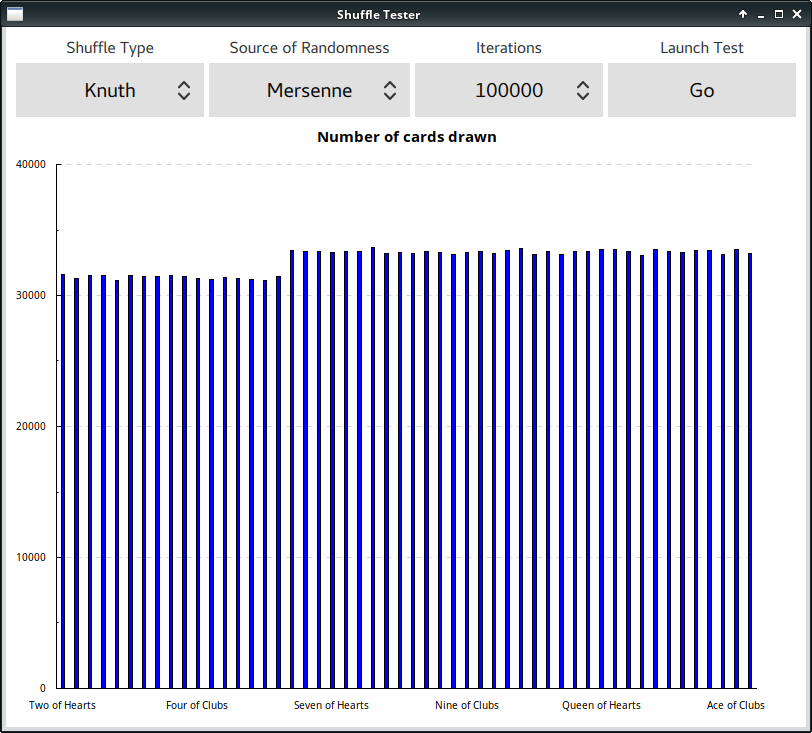
\includegraphics[width=0.8\linewidth]{../images/faultymersenne.png}
    \caption{The Non Uniform Mersenne Distribution}%
    \label{fig:faultymersenne}
\end{figure}

This was due to the random library having no function allowing random numbers
within a range to be generated, and instead a na\"{\i}ve implementation was
used:

\begin{lstlisting}[basicstyle=\footnotesize]
randomFrom0ToN_Mersenne :: Int -> IO Int
randomFrom0ToN_Mersenne n = (`mod` n) <$> M.getStdRandom M.random
\end{lstlisting}

Due to the the values not begin distributed evenly, this resulted in the
above non uniform distribution. This was solved by using an algorithm in which
all the possible values of the random number generator are divided into equal
sized intervals, each representing one of the desired values. For example
if the maximum number the random number generate can create is 11, and the
desired values are a range from 0 to 5, \{0,1\} would be assigned to 0, \{2,3\}
to 1, and so on. The new algorithm is shown below. \parencite{website:reich2011}

\lstinputlisting[firstline=23, lastline=38]
                {\codelocation/server/src/lib/RandomSource.hs}

To an extent this demonstrates how easy it would for poker software to have
biased distributions if rigorous testing procedures were not in place.

A simple way for a malicious actor to generate cards which appear to be random
but actually benefit or hinder a player is to generate cards in a random
way, as in one of the above algorithms, then inspect the generated cards,
and distribute them to players in a specific way to cause the desired effect.
For example, if there were 3 players, and the generated cards were
[Ace, Ace, Seven, Seven, Two, Two], both the aces could be distributed to
the player who has the least chips, whilst the other two players both receive
a seven and two, the statistically worst hand in Texas Hold-Em Poker.

Using this method of rewarding the players with less chips, whilst the overall 
hands and cards generated will be uniform, the cards dealt to each player 
will not be. This could still be measured, but is harder to do so. If the
method is repeatedly applied, in that a player will gain chips by being dealt 
favourable hands and lose chips when dealt bad hands, the player would have 
a cycle of good to bad cards dealt to him as his chips decrease and increase, 
and so might be difficult to detect over long periods, as the highs and lows 
would cancel out.

However, this would be possible to detect if a player is particularly good, or
particularly bad. If they are particularly good, and play their bad hands well
to minimise their chip loss, they will over long periods have a non uniform
card distribution due to constantly having more chips than the average player.

Again, this can be mitigated by dealing uniformly distributed cards to all
players, but instead manipulating the table cards, so flops which benefit
the players with less chips' hands. In this way, a good player still receives
the amount of AA hands as a poorer player, but upon having this AA hand will
find that other players achieve three of a kinds, two pairs, flushes etc
with their lower ranked hands.

As you can tell, there are many ways to manipulate the card generation in
harder and harder to detect ways to the casino's benefit. It is for this
reason that casinos must be transparent about their algorithms and allow
for rigorous investigation by standards agencies.
